% ============================================================
% BLOC 3: IMPLEMENTACIÓ  (diapositives 9–12)
% Cada slide: pàgina real de l'aplicació + explicació sota el capó
% ============================================================

% ---  DIAPOSITIVA — Configuració de Sistema  ---
\begin{frame}{Configuració de Sistema \small\textit{1/3}}
  \begin{columns}[T]
    \begin{column}{0.58\textwidth}
      \begin{center}
        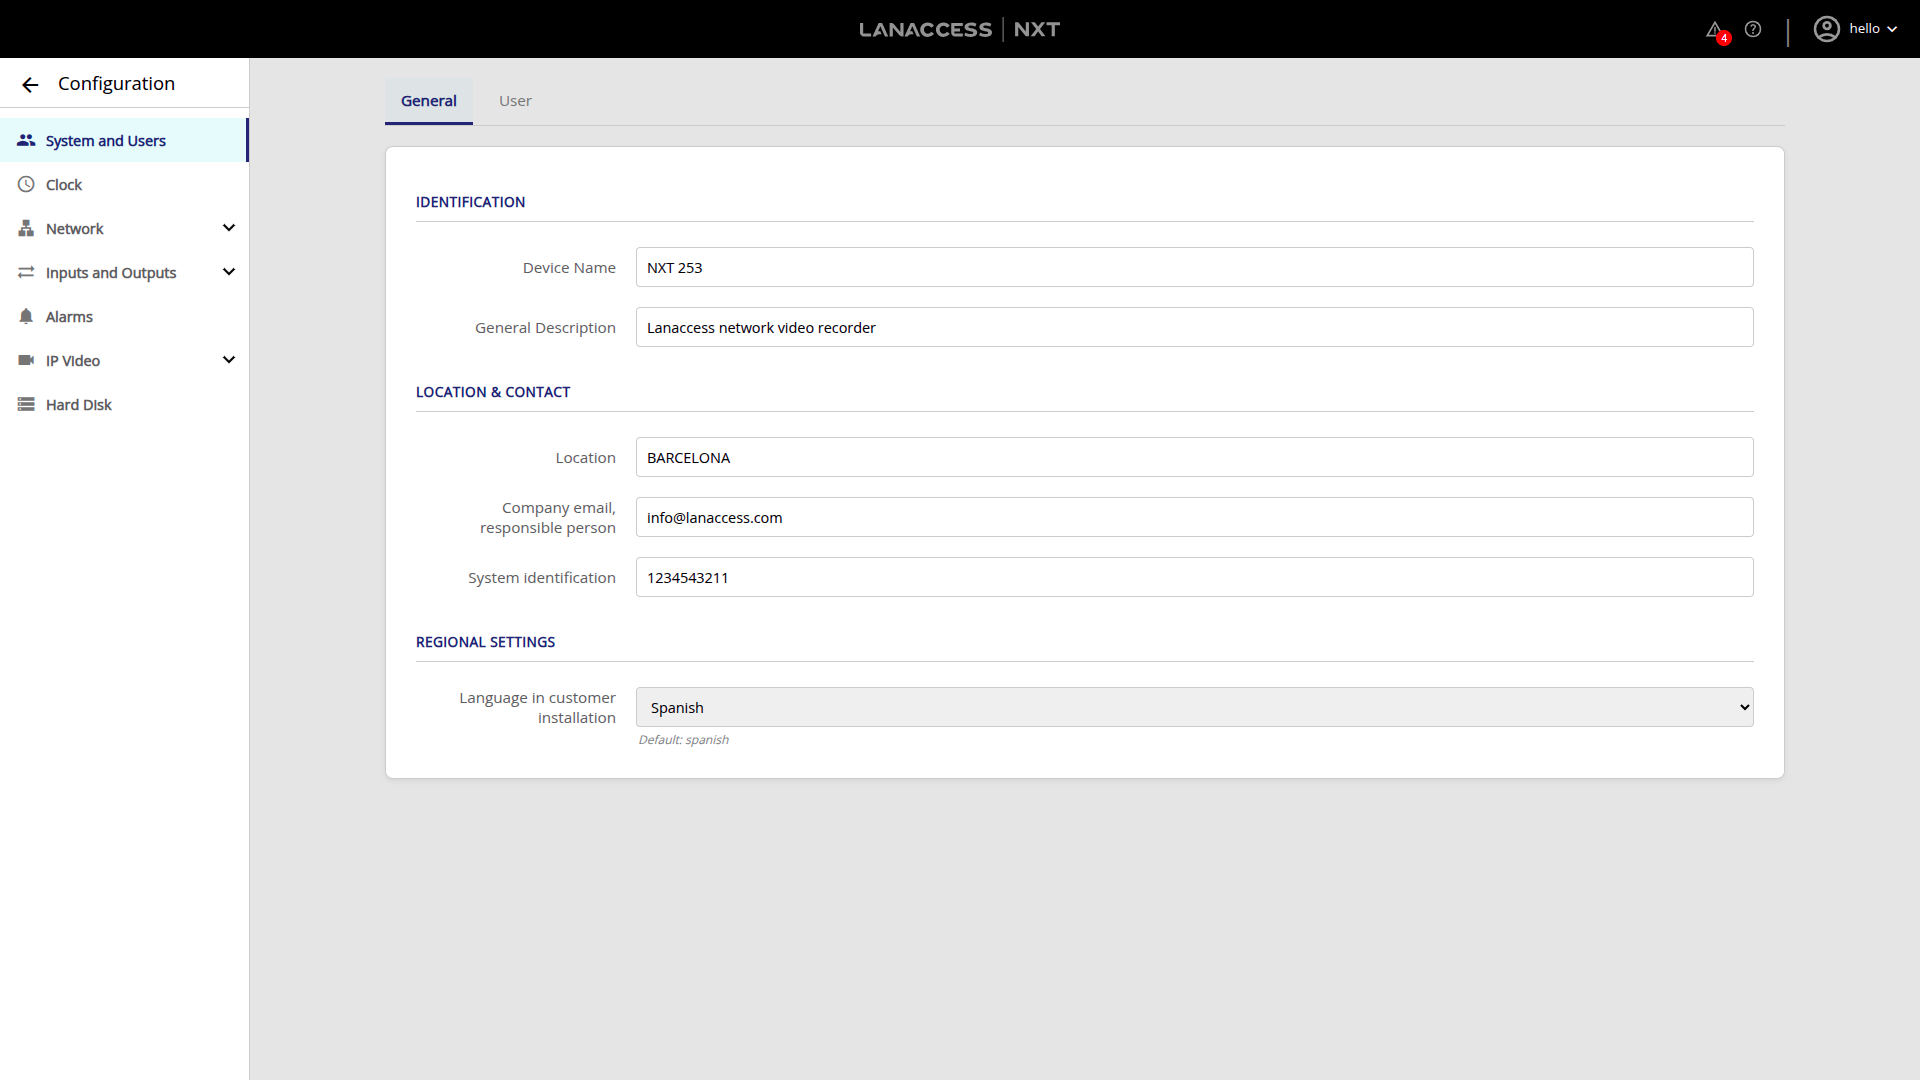
\includegraphics[width=\textwidth, height=0.74\textheight, keepaspectratio]{../figures/interficies/config1.png}
      \end{center}
    \end{column}

    \begin{column}{0.38\textwidth}
      \vspace{0.8em}
      \small El backend envia \textbf{metadades}, no formularis.

      \vspace{0.7em}
      $\Rightarrow$ \texttt{ConfigInputComponent} renderitza \textbf{automàticament}.

      \vspace{0.7em}
      \begin{itemize}
        \item \textbf{10 tipus} de camp $\cdot$ 100\% de la config coberta.
        \item Nou firmware $\Rightarrow$ \textbf{zero canvis} al frontend.
      \end{itemize}
    \end{column}
  \end{columns}

  \note{
    La pantalla que veieu és la configuració d'una càmera IP. L'operador veu un formulari ben estructurat amb checkboxes, desplegables i camps de text. El que és sorprenent és com s'ha construït: Angular no té cap formulari definit al codi. No hi ha cap plantilla HTML que descrigui quins camps han d'existir.

    Quan l'operador obre la configuració, Angular fa un GET al backend i rep un arbre JSON ple de metadades. Cada camp porta un \_type. El component ConfigInputComponent llegeix aquest \_type i renderitza l'element HTML correcte automàticament.

    Hi ha 10 tipus que cobreixen el 100\% de la configuració. L'impacte directe: un NVR amb 20 paràmetres nous en el pròxim firmware és zero canvis al frontend. Zero PR. Zero deploy. El gravador és l'única font de veritat.
  }
\end{frame}

% ---  DIAPOSITIVA — Schema JSON  ---
\begin{frame}[fragile]{Configuració de Sistema \small\textit{2/3}}
  \begin{columns}[T]
    \begin{column}{0.49\textwidth}
      \begin{lstlisting}[style=jsonbox]
{
 "config.video.cam": {
  "{camId}": {
   "_rule": {
    "indexFrom": 0, "indexTo": 151,
    "padding": 3, "fixed": true
   },
   "base": {
    "disabled": {
     "_type": "boolean",
     "_default": "false"
    },
    "ipcamera": {
     "class": {
      "_type": "list",
      "_default": "ONVIF",
      "_allowedValues": [
       "VIVOTEK","ONVIF","RTSP"
      ]
     }, ...
      \end{lstlisting}
    \end{column}

    \begin{column}{0.49\textwidth}
      \begin{lstlisting}[style=jsonbox]
     "connection": {
      "address": {
       "_type": "ipaddr",
       "_default": "0.0.0.0"
      },
      "port": { "config": {
       "_type": "numeric",
       "_default": 80,
       "_minValue": 1,
       "_maxValue": 65535
      }}
     },
     "account": {
      "password": {
       "_type": "password",
       "_maxLength": 24,
       "_policyLevel": 0
      }
     }
    }}}}}
      \end{lstlisting}
    \end{column}
  \end{columns}

  \note{
    Aquí veiem el schema real que envia el backend. La clau arrel és el node de configuració: config.video.cam. La clau \{camId\} és dinàmica: el backend substitueix el patró per cada índex de càmera, del 0 al 151, definit per \_rule. Això indexa tots els camps sense duplicar la definició.

    Fixeu-vos en els cinc tipus que apareixen aquí. disabled és boolean: renderitza un checkbox. class és list: renderitza un select amb exactament les opcions d'\_allowedValues, sense cap codi addicional. address és ipaddr: un input amb validació regex d'IP. port és numeric, amb \_minValue i \_maxValue que Angular trasllada directament als atributs HTML5 min i max. I password és un input de tipus password amb restriccions de longitud i política de seguretat.

    Cap d'aquesta lògica és codi Angular específic per a càmeres. És declaració pura: el schema diu QUÈ és cada camp, el ConfigInputComponent sap COM renderitzar-ho. Cinc tipus aquí, deu en total, cobrint el 100\% del sistema.
  }
\end{frame}

% ---  DIAPOSITIVA — Config Lock Pessimista  ---
\begin{frame}[fragile]{Configuració de Sistema \small\textit{3/3}}
  \begin{columns}[T]
    \begin{column}{0.46\textwidth}
      \small\textbf{POST /lock $\to$ token d'escriptura exclusiva:}
      \vspace{0.3em}

      \begin{lstlisting}[style=jsonbox]
{
  "path":      "config",
  "token":     "a1b2c3d4e5f6g7h8i9j0k1l2m3n4o5p6",
  "expiresIn": 60,
  "seed":      "8b9f27cda0134e7f8a9bcdef01234567"
}\end{lstlisting}

      \vspace{0.4em}
      \begin{itemize}
        \item Token: injectat per \textbf{interceptor}.
        \item Renovació cada \texttt{expiresIn/2} segons.
        \item Sessió concurrent: \textbf{HTTP 423} $\to$ mode lectura.
        \item Sortir: expira i s'allibera sol.
      \end{itemize}
    \end{column}

    \begin{column}{0.50\textwidth}
      \begin{center}
        \vspace{-2cm}
        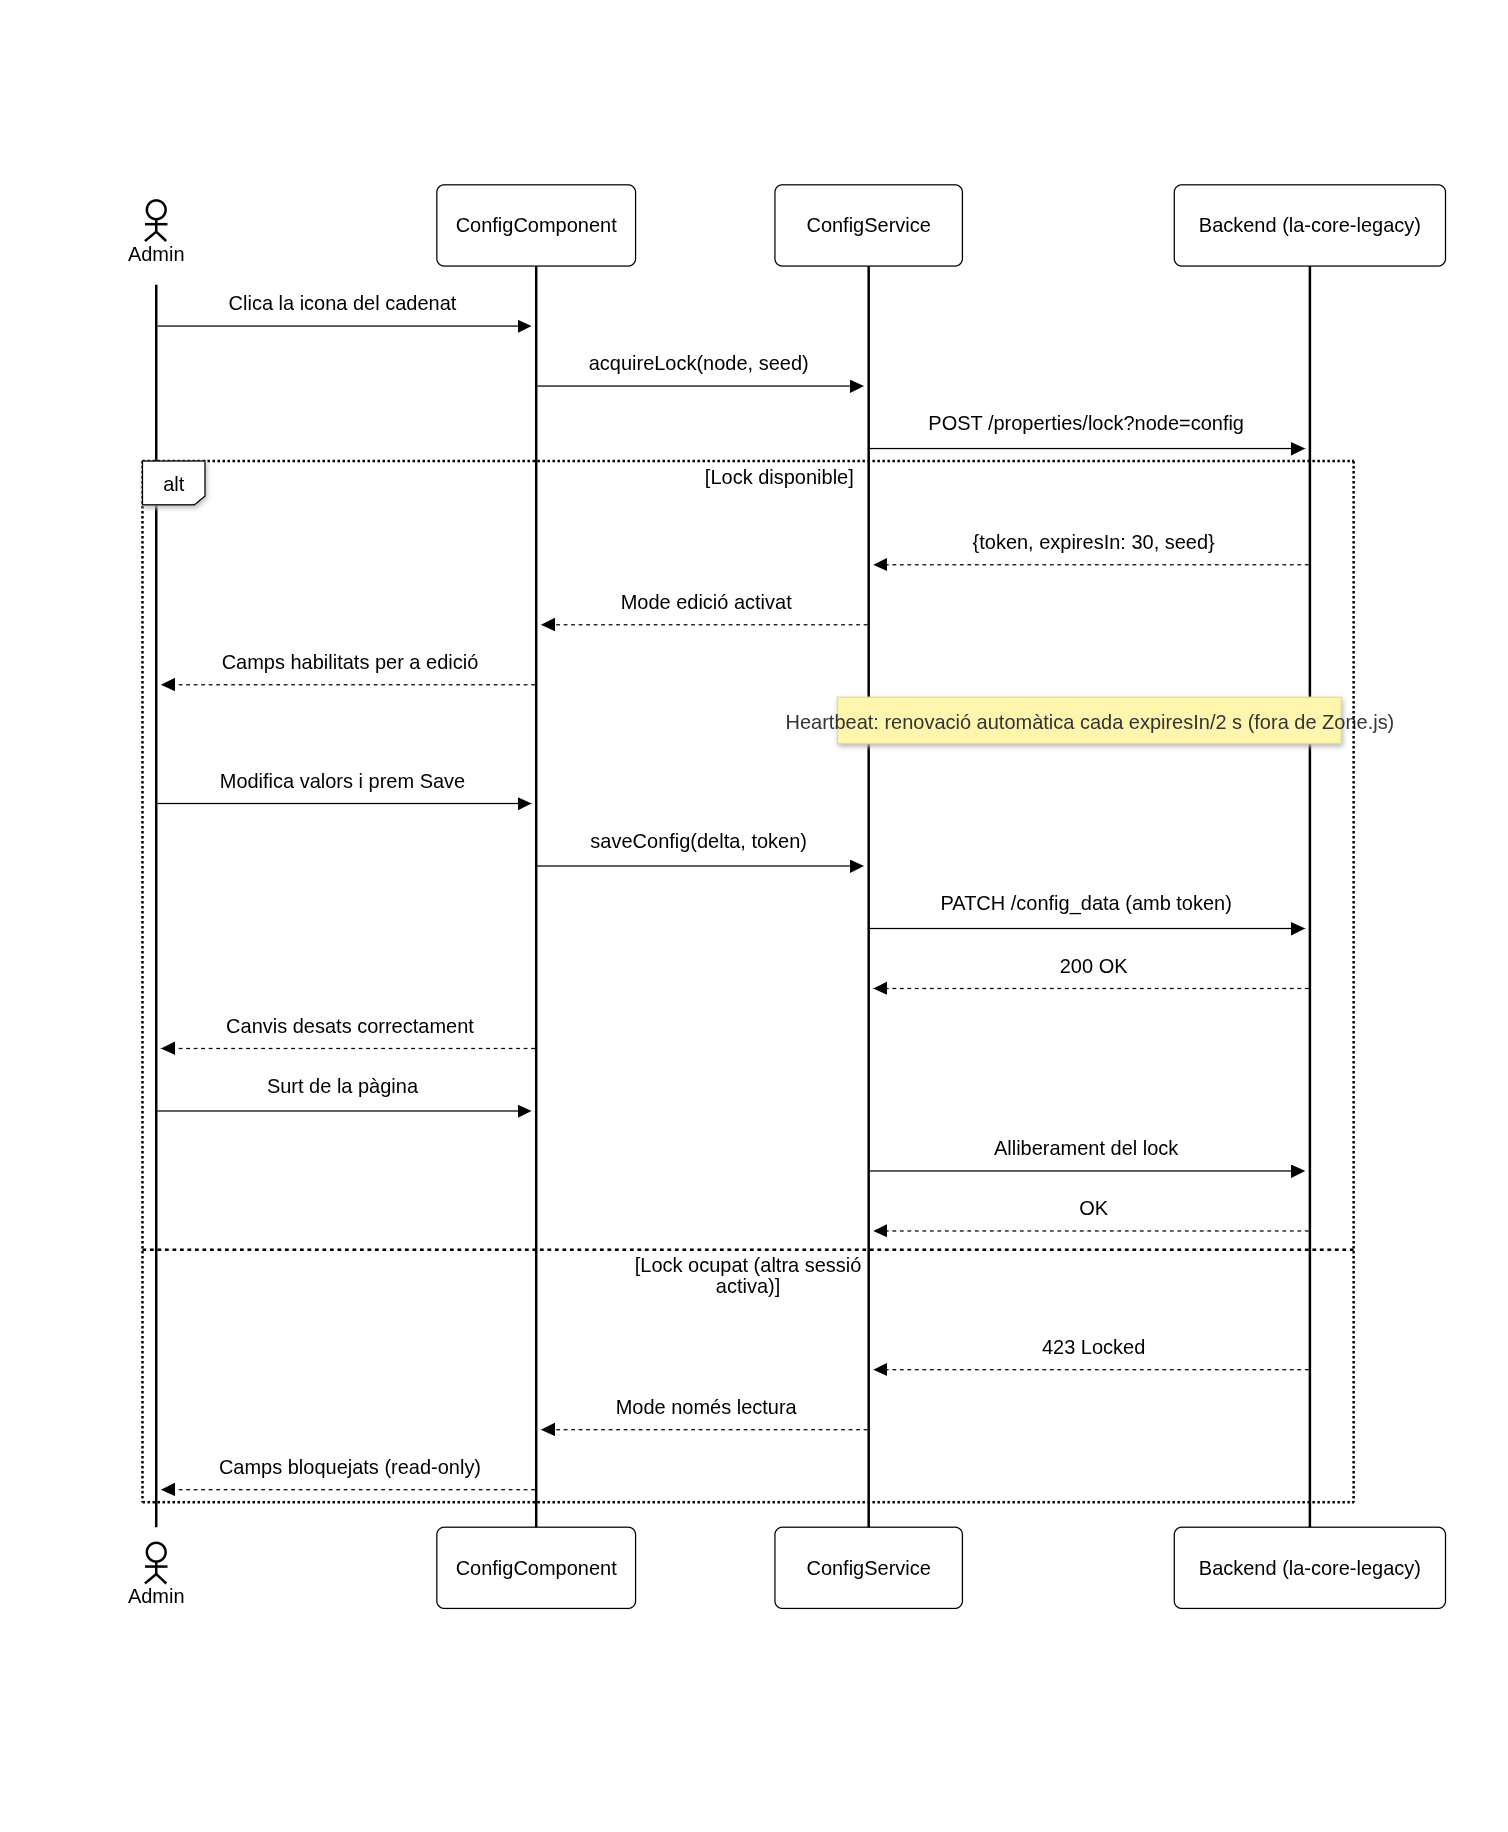
\includegraphics[width=\textwidth, height=1\textheight, keepaspectratio]{../figures/diagrames/seq_config_lock.png}
      \end{center}
    \end{column}
  \end{columns}

  \note{
    La concurrència és un problema real: un tècnic de camp i un administrador poden obrir la configuració simultàniament i sobreescriure els canvis de l'altre. El Pessimistic Lock ho elimina completament.

    En entrar a configuració, Angular fa automàticament POST a /lock. El servidor retorna un token de 32 caràcters i un temps de vida: 60 o 120 segons depenent del node. A partir d'aquí, tot PUT a /config.* porta el token: no ho fa el component ni el servei, sinó un interceptor HTTP global transparent. Cap component sap de la seva existència.

    La renovació és cada expiresIn/2 fora de Zone.js per no disparar cicles de detecció de canvis innecessaris. Si un segon operador intenta adquirir el lock: HTTP 423 Locked, i el frontend el posa automàticament en mode lectura via un Signal. Si el tècnic tanca l'ordinador, el lock expira sol i es lliura sense cap intervenció manual.
  }
\end{frame}

% ---  DIAPOSITIVA 9 — Pàgina de Directe  ---
\begin{frame}{Vídeo en Directe}
  \begin{columns}[T]
    \begin{column}{0.54\textwidth}
      \begin{center}
        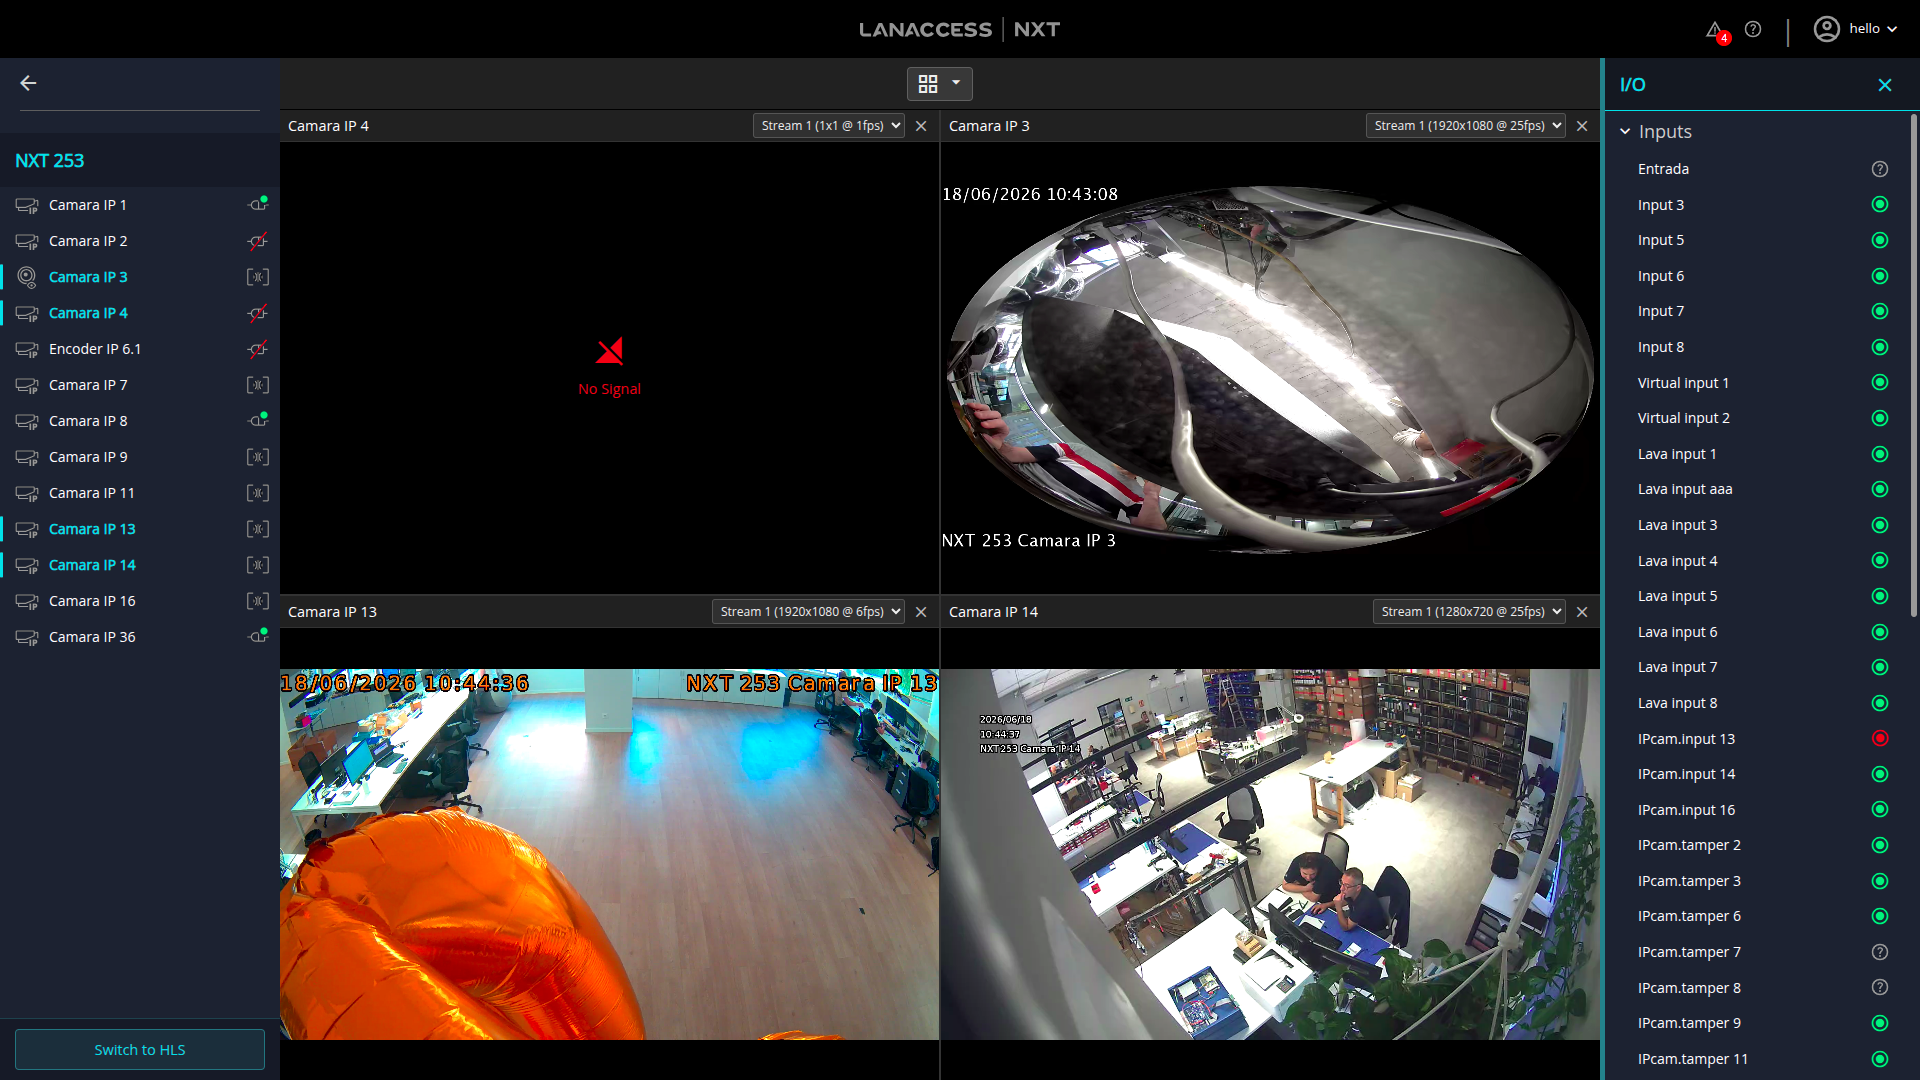
\includegraphics[width=\textwidth, height=0.6\textheight, keepaspectratio]{../figures/interficies/cameras.png}
      \end{center}
    \end{column}

    \begin{column}{0.43\textwidth}
      \textbf{Sota el capó:}
      \begin{itemize}
        \item \textbf{WHEP} (RFC 9716): UDP/SRTP + DTLS + ICE.
        \item Latència \textbf{150--300 ms} vs 800--2000 ms (ActiveX).
        \item Fallback \textbf{HLS} en $\leq$ 5 s (UDP bloquejat).
        \item \textbf{Angular Signals}: \textbf{35\% menys CPU} (i3-8100T).
      \end{itemize}
    \end{column}
  \end{columns}

  \note{
    Quan l'operador obre la pàgina de directe, Angular fa un POST a l'endpoint WHEP de cada càmera. WHEP, el WebRTC HTTP Egress Protocol, estandaritza la negociació amb una sola crida HTTP. A partir d'aquí s'estableix la connexió UDP directa amb xifrat DTLS i ICE per a la travessia de NATs.

    El resultat: 150 a 300 mil·lisegons de latència. L'antiga plataforma ActiveX basada en RTSP oscil·lava entre 800 ms i 2 segments. Els rangs no se solapen: el pitjor cas de WebRTC és millor que el millor cas d'ActiveX.

    Si UDP és bloquejat per un firewall corporatiu, Angular detecta el timeout en 5 segments i commuta automàticament a HLS. L'operador mai veu un error.

    I gràcies als Angular Signals, quan arriba un frame de la càmera 3, s'actualitza únicament el component d'aquella càmera. Zone.js hauria rellegit tot el DOM. Resultat mesurat: 35\% menys CPU en un terminal Intel Core i3-8100T sota Windows 10 IoT, amb 4 càmeres en continu.
  }
\end{frame}

% ---  DIAPOSITIVA 10 — Pàgina de Gravacions  ---
\begin{frame}{Gravacions}
  \begin{columns}[T]
    \begin{column}{0.54\textwidth}
      \begin{center}
        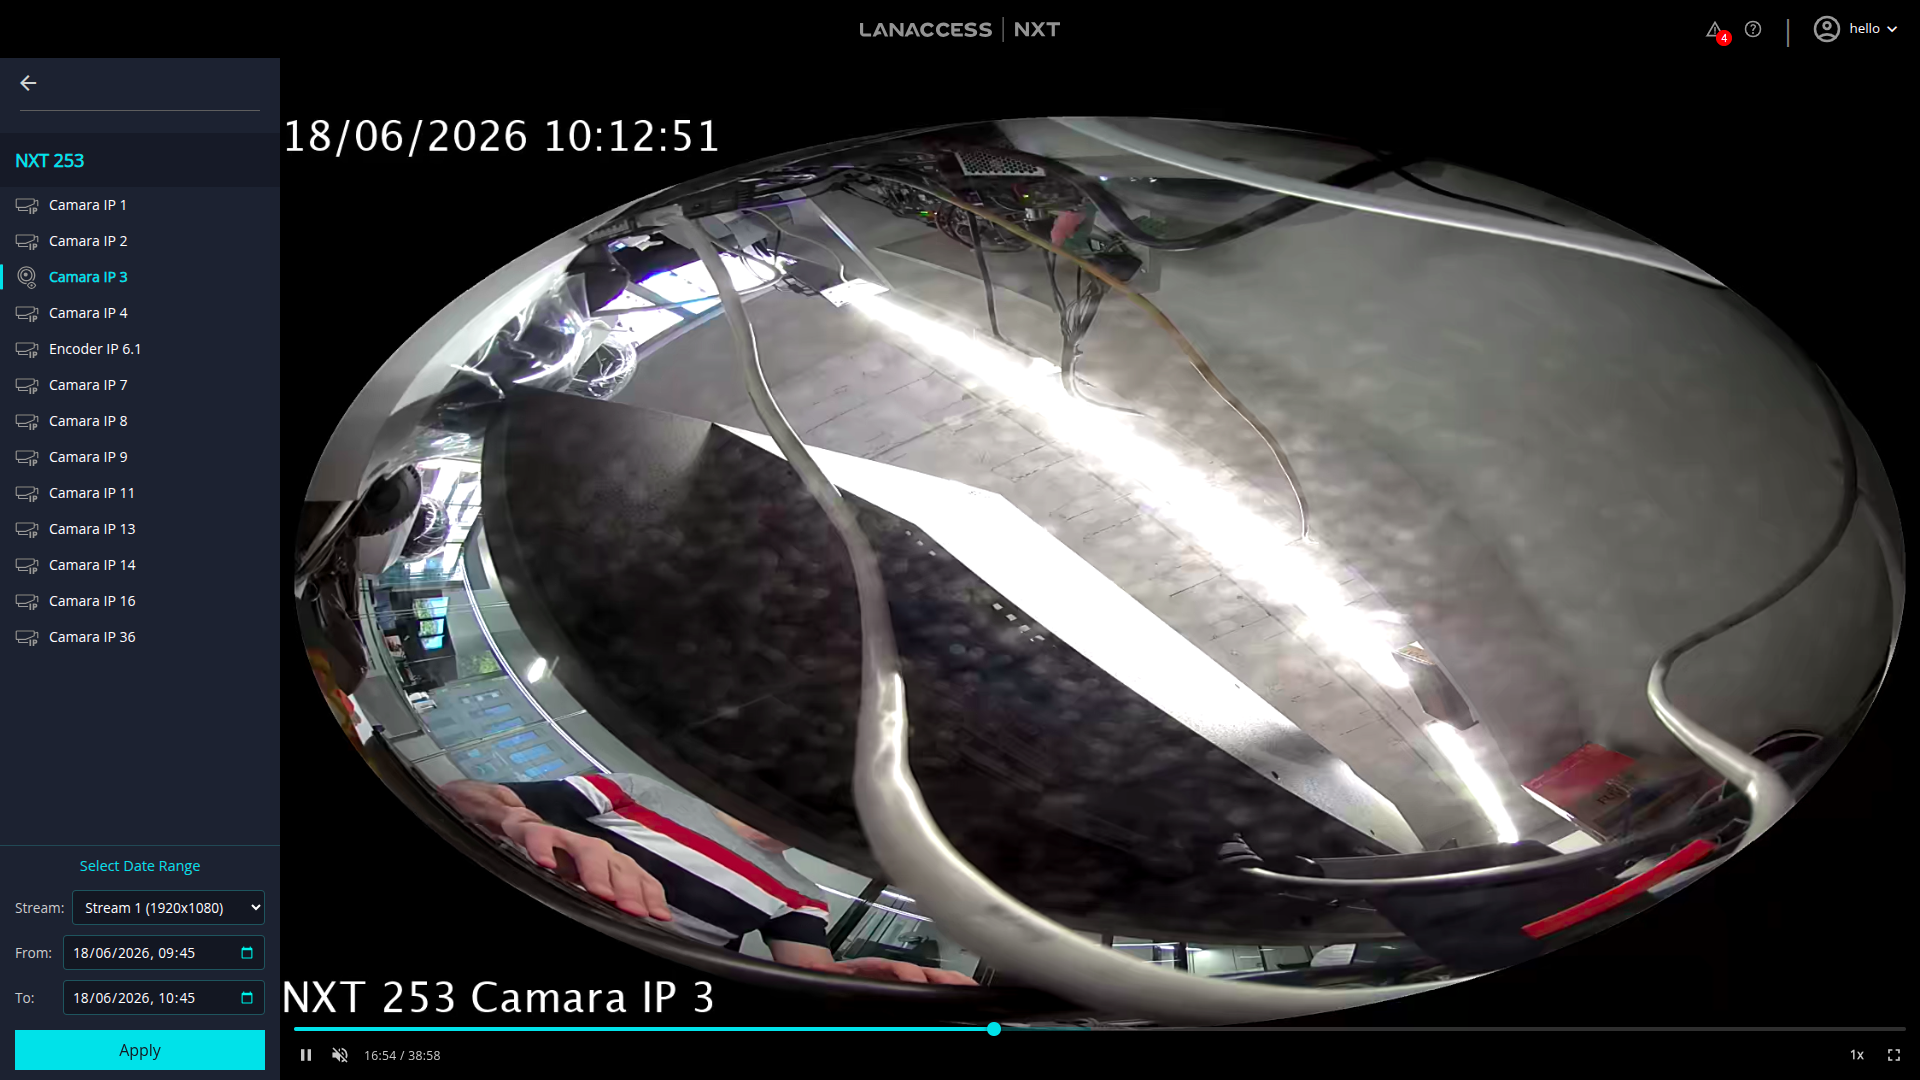
\includegraphics[width=\textwidth, height=0.6\textheight, keepaspectratio]{../figures/interficies/recordings.png}
      \end{center}
    \end{column}

    \begin{column}{0.43\textwidth}
      \small\textbf{Sota el capó:}
      \begin{itemize}
        \item \textbf{FS2}: format propietari, cap reproductor web.
        \item \textbf{Trans-muxing}: FS2 $\to$ SPS/PPS/VPS $\to$ MPEG-TS.
        \item $\neq$ transcoding: embolcall, no bitstream. \textbf{CPU $\approx$ 0}.
        \item \textbf{H.265}: \textbf{50\% menys disc} que H.264.
      \end{itemize}
    \end{column}
  \end{columns}

  \note{
    L'operador selecciona un segment temporal i reprodueix. El que veu és fluid; el que passa al darrere és complex.

    Les gravacions al disc estan en format FS2 propietari: blocs bruts sense contenidor, sense capçaleres estàndard. Cap reproductor web pot llegir-los directament.

    El microservei la-video-engine fa trans-muxing en temps real: llegeix el bloc FS2, recupera les capçaleres SPS, PPS i VPS que contenen la informació de descodificació ---que de vegades no estan en cada segment sinó que cal recuperar del keyframe anterior---, i les injecta davant del bitstream. Finalment, empaqueta tot en format MPEG-TS per a HLS.

    La clau és que no estem recomprimint el vídeo, només canviem l'embolcall. La CPU del gravador no s'ha d'esforçar en operacions de codificació. H.265 ocupa un 50\% menys de disc que H.264 per la mateixa qualitat: factor crític en gravadors que funcionen les 24 hores.
  }
\end{frame}

% ---  DIAPOSITIVA 11 — Gestió Reactiva d'Alarmes  ---
\begin{frame}{Alarmes}
  \begin{columns}[T]
    \begin{column}{0.45\textwidth}
      \textbf{Push i Persistència:}
      \begin{itemize}
        \item \textbf{WebSocket push}: sensor $\to$ operadors en temps real.
        \item Reconnexió: \textbf{backoff exponencial}.
        \item \textbf{remote\_vfs}: SQLite via Unix Domain Socket.
        \item Atomicitat: alineació a \textbf{512 B}.
        \item Mode \textbf{WAL}: ACID verificat en talls elèctrics.
      \end{itemize}
    \end{column}

    \begin{column}{0.5\textwidth}
      \begin{center}
        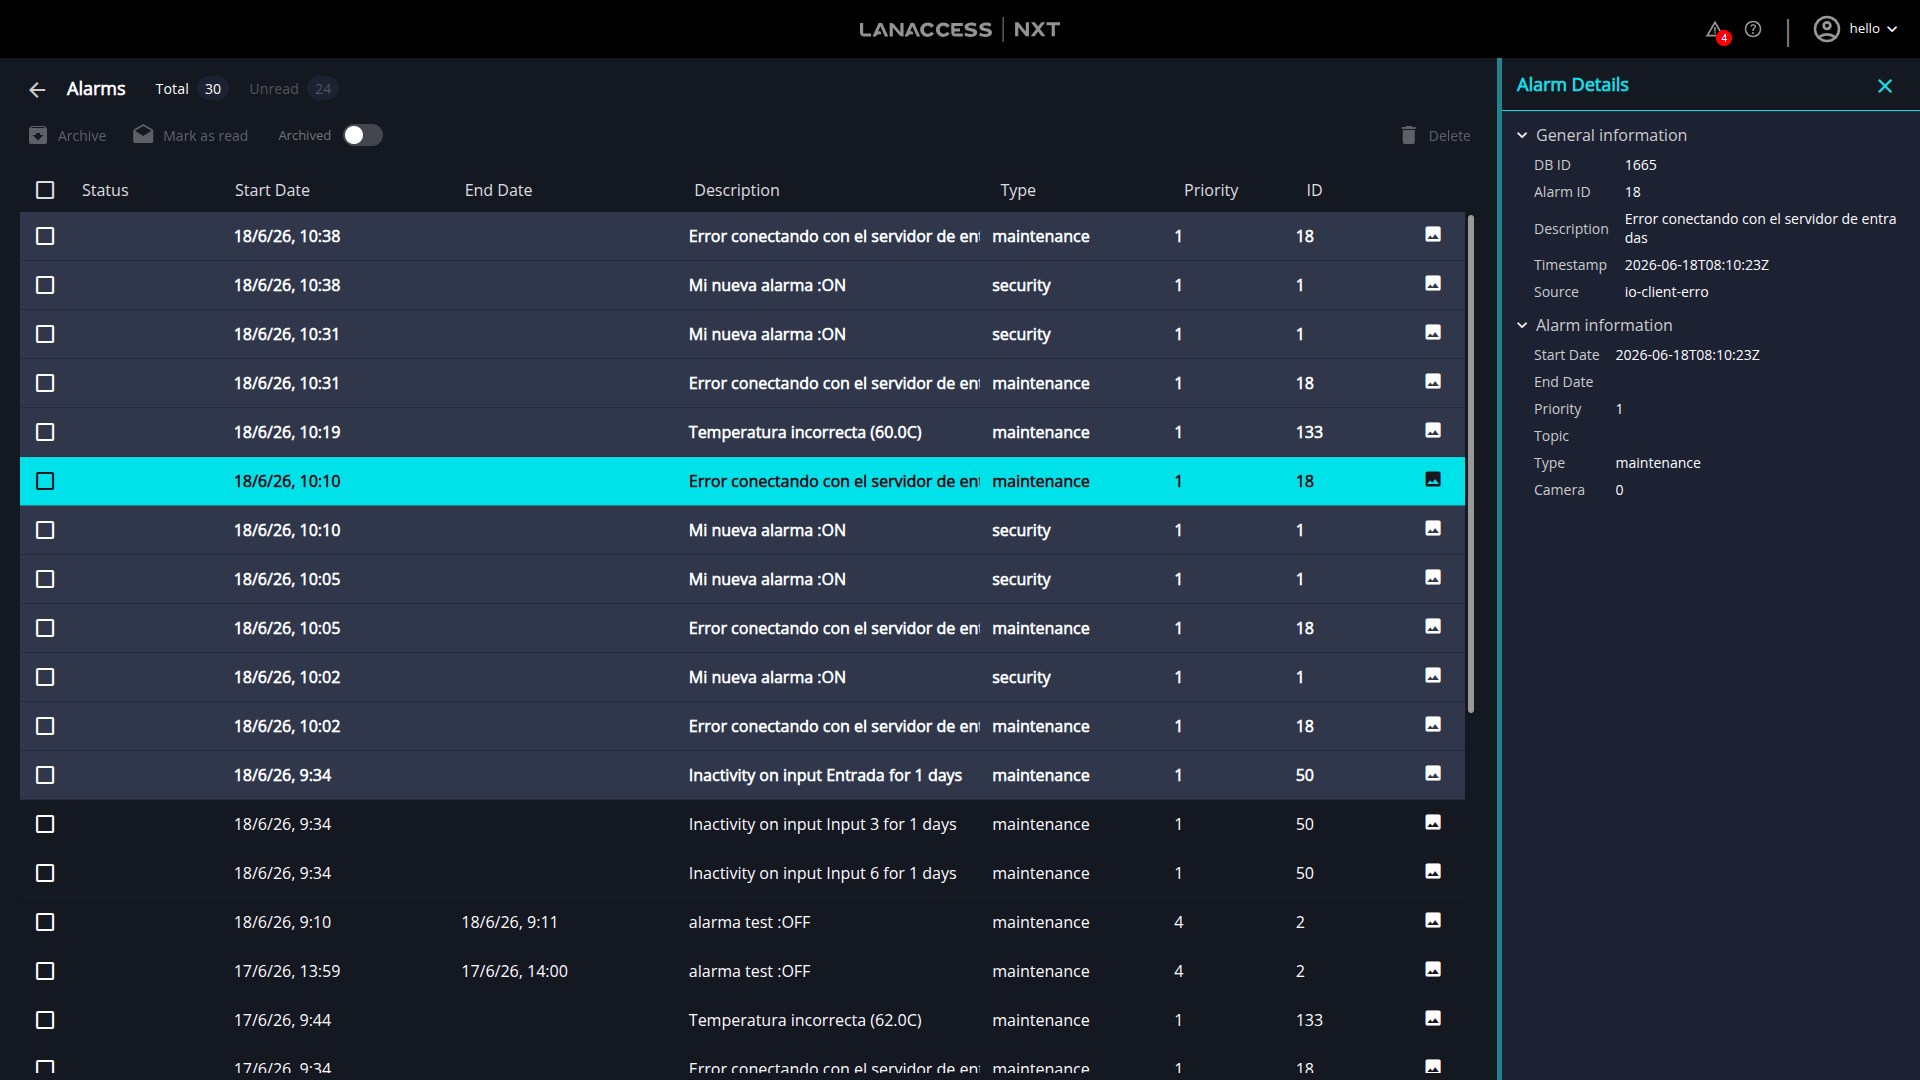
\includegraphics[width=\textwidth, height=0.7\textheight, keepaspectratio]{../figures/interficies/alarms.png}
      \end{center}
    \end{column}
  \end{columns}

  \note{
    El sistema d'alarmes requeria resoldre dos problemes independents: la notificació en temps real i la persistència davant de talls de corrent.

    Per a la notificació: connexió WebSocket segura persistent. Quan un sensor salta, la-core-alarm ho emet immediatament per WebSocket a tots els operadors connectats. Gràcies als Signals, s'actualitza únicament la icona de l'alarma afectada. Si la connexió cau, la reconnexió automàtica amb backoff exponencial protegeix la CPU del gravador d'allaus de reconnexions simultànies.

    Per a la persistència: el driver VFS personalitzat remote\_vfs redirigeix totes les operacions d'SQLite a través d'un Unix Domain Socket cap al la-db-engine, l'únic procés amb permisos d'escriptura al disc. Les escriptures s'alineen a sectors de 512 bytes per garantir atomicitat davant de talls de corrent sobtats. El mode WAL ofereix garanties ACID completes, verificades en simulacions de tall elèctric forçat.
  }
\end{frame}
